\documentclass[a4paper,12pt,obeyspaces,spaces,hyphens]{article}

\def \trainingtitle{Embedded Linux system development training}
\def \trainingduration{On-site training, 4 days}
\def \agendalanguage{english}
\def \training{embedded-linux}

\usepackage{agenda}

\begin{document}

\feshowtitle

\feagendasummaryitem{Title}{
  {\bf \trainingtitle{}}
}
\feagendasummaryitem{Training objectives}{
  \begin{itemize}
  \item Understand the overall architecture of Embedded Linux
    systems.
  \item Understand the role and internals of a cross-compilation toolchain
    and setup your own.
  \item Understand the booting process of embedded systems, the main
    bootloaders, and setup your own bootloader.
  \item Understand the role and overall architecture of Linux
    kernel, how to configure, build and install it on your embedded
    system.
  \item Understand the principle and contents of a Linux root
    filesystem, and create your own Linux root filesystem from
    scratch.
  \item Discover the different filesystem for block storage devices,
    and use them on your embedded system.
  \item Discover major open-source software components for embedded
    systems, understanding licensing constraints, how to integrate
    and cross-compile third-party software components, and
    experiment cross-compilation of open-source libraries.
  \item Discover the main embedded Linux build systems, and
    experiment one of them.
  \item Understand the principles and tools for application
    development and debugging on embedded Linux systems.
  \end{itemize}
}
\feagendasummaryitem{Duration}{
  {\bf Four} days - 32 hours (8 hours per day).
}
\onsitepedagogics{50}{50}{embedded-linux-4d}
\feagendasummaryitem{Trainer}{
  One of the engineers listed on:
  \newline \url{https://bootlin.com/training/trainers/}
}
\feagendasummaryitem{Language}{
  Oral lectures: English or French.
  \newline Materials: English.
}
\feagendasummaryitem{Audience}{
  People developing devices using the Linux kernel
  \newline People supporting embedded Linux system developers.
}
\feagendasummaryitem{Prerequisites}{
  \begin{itemize}
    \prerequisitecommandline
    \prerequisiteenglish
  \end{itemize}
}
\feagendasummaryitem{Alternative version}{
  Full version of the Embedded Linux
  system development course, ({\bf 5 days long}) with 2 additional
  half days with practical labs:
  \begin{itemize}
  \item Flash filesystems
  \item Real time
  \end{itemize}
  Practical labs using a Microchip SAMA5D3 Xplained board
  \url{https://bootlin.com/doc/training/embedded-linux/embedded-linux-agenda.pdf}.
}
\ferequiredequipmentonsite{}
\certificate{}
\disabilities{}

\feagendatwocolumn
{Hardware}
{
  Using the {\em STMicroelectronics STM32MP157D-DK1 Discovery board} in all
  practical labs. This board features:

  \begin{itemize}
  \item STM32MP157D dual ARM Cortex-A7 processor
  \item USB-C powered
  \item 512 MB DDR3L RAM
  \item Gigabit Ethernet port
  \item 4 USB 2.0 host ports
  \item 1 USB-C OTG port
  \item 1 Micro SD slot
  \item On-board ST-LINK/V2-1 debugger
  \item Arduino Uno v3-compatible header
  \item Audio codec
  \item Misc: buttons, LEDs
  \end{itemize}
}
{}
{
  \begin{center}
    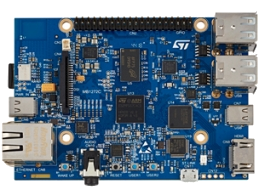
\includegraphics[height=5cm]{../slides/discovery-board-dk1/discovery-board-dk1.png}
  \end{center}
}

\section{Day 1 - Morning}

\feagendaonecolumn
{Lecture - Introduction to embedded Linux}
{
  \begin{itemize}
  \item Introduction to Free Software
  \item Reasons for choosing Free Software in embedded operating systems
  \item Example embedded systems running Linux
  \item CPU, RAM and storage requirements
  \item Choosing a hardware platform
  \item System architecture: main components
  \item Embedded system development tasks
  \end{itemize}
}
\\
\feagendatwocolumn
{Lecture - Embedded Linux development environment}
{
  \begin{itemize}
  \item Operating system and tools to use on the development
        workstation for embedded Linux development.
  \end{itemize}
}
{Lecture - Cross-compiling toolchain and C library}
{
  \begin{itemize}
  \item What's inside a cross-compiling toolchain
  \item Choosing the target C library
  \item What's inside the C library
  \item Ready to use cross-compiling toolchains
  \item Building a cross-compiling toolchain with automated tools.
  \end{itemize}
}

\section{Day 1 - Afternoon}
\feagendatwocolumn
{Lab - Cross compiling toolchain}
{
  \begin{itemize}
  \item Configuring Crosstool-NG
  \item Executing it to build a custom uClibc toolchain.
  \end{itemize}
}
{Lecture - Bootloaders}
{
  \begin{itemize}
  \item Available bootloaders
  \item Bootloader features
  \item Installing a bootloader
  \item Detailed study of U-Boot
  \end{itemize}
}
\\

\feagendatwocolumn
{Lab - Bootloader and U-boot}
{
  {\em Using the STM32MP157D-DK1 Discovery board}
  \begin{itemize}
  \item Set up serial communication with the board.
  \item Configure, compile and install the first-stage bootloader
        and U-Boot on the Discovery board.
  \item Become familiar with U-Boot environment and commands.
  \item Set up TFTP communication with the board. Use TFTP U-Boot commands.
  \end{itemize}
}
{Lecture - Linux kernel}
{
  \begin{itemize}
  \item Role and general architecture of the Linux kernel
  \item Features available in the Linux kernel,
        with a focus on features useful for embedded systems
  \item Kernel user interface
  \item Getting the sources
  \item Linux kernel release process. Long Term Support versions.
  \item Using the patch command
  \end{itemize}
}
\\

\section{Day 2 - Morning}

\feagendatwocolumn
{Lab - Kernel sources}
{
  \begin{itemize}
  \item Downloading kernel sources
  \item Apply kernel patches
  \end{itemize}
}
{Lecture – Configuring and compiling a Linux kernel}
{
  \begin{itemize}
  \item Kernel configuration.
  \item Using ready-made configuration files for specific architectures and boards.
  \item Kernel compilation.
  \item Generated files.
  \item Using kernel modules
  \end{itemize}
}

\feagendaonecolumn
{Lab - Kernel cross-compiling and booting}
{
  {\em Using the STM32MP157D-DK1 Discovery board}
  \begin{itemize}
  \item Configuring the Linux kernel and cross-compiling it for the ARM board.
  \item Downloading your kernel on the board through U-boot's tftp client.
  \item Booting your kernel from RAM.
  \item Copying the kernel to flash and booting it from this location.
  \item Storing boot parameters in flash and automating kernel booting from flash.
  \end{itemize}
}

\section{Day 2 - Afternoon}

\feagendatwocolumn
{Lecture – Root filesystem in Linux}
{
  \begin{itemize}
  \item Filesystems in Linux.
  \item Role and organization of the root filesystem.
  \item Location of the root filesystem: on storage, in memory,
        from the network.
  \item Device files, virtual filesystems.
  \item Contents of a typical root filesystem.
  \end{itemize}
}
{Lecture - BusyBox}
{
  \begin{itemize}
  \item Detailed overview. Detailed features.
  \item Configuration, compiling and deploying.
  \end{itemize}
}

\feagendaonecolumn
{Lab – Tiny root filesystem built from scratch with BusyBox}
{
  {\em Using the STM32MP157D-DK1 Discovery board}
  \begin{itemize}
  \item Now build a basic root filesystem from scratch for your ARM system
  \item Setting up a kernel to boot your system on a workstation
        directory exported by NFS
  \item Passing kernel command line parameters to boot on NFS
  \item Creating the full root filesystem from scratch.
        Populating it with BusyBox based utilities.
  \item Creating device files and booting the virtual system.
  \item System startup using BusyBox /sbin/init
  \item Using the BusyBox http server.
  \item Controlling the target from a web browser on the PC host.
  \item Setting up shared libraries on the target and compiling
        a sample executable.
  \end{itemize}
}

\section{Day 3 - Morning}

\feagendatwocolumn
{Lecture - Block filesystems}
{
  \begin{itemize}
  \item Filesystems for block devices.
  \item Usefulness of journaled filesystems.
  \item Read-only block filesystems.
  \item RAM filesystems.
  \item How to create each of these filesystems.
  \item Suggestions for embedded systems.
  \end{itemize}
}
{Lab - Block filesystems}
{
  {\em Using the STM32MP157D-DK1 Discovery board}
  \begin{itemize}
  \item Creating partitions on your block storage
  \item Booting a system with a mix of filesystems: SquashFS for
	applications, ext3 for configuration and user data, and
	tmpfs for temporary system files.
  \end{itemize}
}

\section{Day 3 - Afternoon}

\feagendaonecolumn
{Lecture – Leveraging existing open-source components in your system}
{
  \begin{itemize}
  \item Reasons for leveraging existing components.
  \item Find existing free and open source software components.
  \item Choosing the components.
  \item The different free software licenses and their requirements.
  \item Overview of well-known typical components used in
        embedded systems: graphical libraries and systems
        (framebuffer, Gtk, Qt, etc.), system utilities,
        network libraries and utilities, multimedia libraries, etc.
  \item System building: integration of the components.
  \end{itemize}
}

\feagendatwocolumn
{Lecture – Cross-compiling applications and libraries}
{
  \begin{itemize}
  \item Configuring, cross-compiling and installing applications and libraries.
  \item Details about the build system used in most open-source components.
  \item Overview of the common issues found when using these components.
  \end{itemize}
}
{Lab – Cross-compiling applications and libraries}
{
  {\em If enough time left}
  \begin{itemize}
  \item Building a system with audio libraries and a sound player application.
  \item Manual compilation and installation of several free software packages.
  \item Learning about common techniques and issues.
  \end{itemize}
}

\section{Day 4 - Morning}

\feagendatwocolumn
{Lecture - Embedded system building tools}
{
  \begin{itemize}
  \item Review of existing system building tools.
  \item Buildroot example.
  \end{itemize}
}
{Lab - System build with Buildroot}
{
  {\em Using the STM32MP157D-DK1 Discovery board}
  \begin{itemize}
  \item Using Buildroot to rebuild the same system as in the previous lab.
  \item Seeing how easier it gets.
  \item Optional: add a package to Buildroot.
  \end{itemize}
}

\section{Day 4 - Afternoon}

\feagendaonecolumn
{Lecture - Application development and debugging}
{
  \begin{itemize}
  \item Programming languages and libraries available.
  \item Overview of the C library features for application development.
  \item Build system for your application,
        how to use existing libraries in your application.
  \item Debuggers. Debugging remote applications with gdb and gdbserver.
        Post-mortem debugging with core files.
  \item Code checkers, memory checkers, profilers.
  \end{itemize}
}

\feagendaonecolumn
{Lab – Application development and debugging}
{
  {\em On the STM32MP157D-DK1 Discovery board}
  \begin{itemize}
  \item Develop and compile an application relying on the ncurses library
  \item Using strace, ltrace and gdbserver to debug a crappy application
        on the remote system.
  \item Post mortem analysis: exploit a {\em core dump} to find out where an application
        crashed.
  \end{itemize}
}

\end{document}

